\documentclass[xga]{xdvislides}
\usepackage[landscape]{geometry}
\usepackage{graphics}
\usepackage{graphicx}
\usepackage{colordvi}

\begin{document}
\setfontphv

%%% Headers and footers
\lhead{\slidetitle}                               % default:\lhead{\slidetitle}
\chead{CS631 - Advanced Programming in the UNIX Environment}% default:\chead{\relax}
\rhead{Slide \thepage}                       % default:\rhead{\sectiontitle}
\lfoot{\Gray{HTTP, Coding Practices}}% default:\lfoot{\slideauthor}
\cfoot{\relax}                               % default:\cfoot{\relax}
\rfoot{\Gray{\today}}

\newcommand{\smallish}{\fontsize{15}{20}\selectfont}

\vspace*{\fill}
\begin{center}
	\Hugesize
		CS631 - Advanced Programming in the UNIX Environment\\ [1em]
		HTTP; Coding Practices\\ [1em]
	\hspace*{5mm}\blueline\\ [1em]
	\Normalsize
		Department of Computer Science\\
		Stevens Institute of Technology\\
		Jan Schaumann\\
		\verb+jschauma@stevens.edu+
		\verb+https://www.cs.stevens-tech.edu/~jschauma/631/+
\end{center}
\vspace*{\fill}

\subsection{HTTP: Hypertext}
\begin{center}
	\includegraphics[scale=0.9]{pics/http-proposal-detail.eps} \\
	\vspace{.5in}
	\verb+http://is.gd/JnZaN6+
\end{center}

\subsection{HTTP}
\vspace{.5in}
\begin{center}
	\Huge
	Hypertext Transfer Protocol
	\\
	\vspace{.5in}
	RFC2616
\end{center}
\Normalsize

\subsection{HTTP}
\vspace{.5in}
\begin{center}
	\Huge
	HTTP is a request/response protocol.
\end{center}
\Normalsize

\subsection{The Hypertext Transfer Protocol}
HTTP is a request/response protocol:
\begin{enumerate}
	\item client sends a request to the server
	\item server responds
\end{enumerate}

\subsection{The Hypertext Transfer Protocol}
HTTP is a request/response protocol:
\begin{enumerate}
	\item client sends a request to the server
		\begin{itemize}
			\item request method
			\item URI
			\item protocol version
			\item request modifiers
			\item client information
		\end{itemize}
	\item server responds
\end{enumerate}

\subsection{HTTP: A client request}
\vspace*{.5in}
\\
\Hugesize
\begin{center}
\begin{verbatim}
$ telnet www.google.com 80
Trying 173.194.75.147...
Connected to www.google.com.
Escape character is '^]'.
GET / HTTP/1.0
\end{verbatim}
\end{center}
\Normalsize
\vspace*{\fill}


\subsection{The Hypertext Transfer Protocol}
HTTP is a request/response protocol:
\begin{enumerate}
	\item client sends a request to the server
		\begin{itemize}
			\item request method
			\item URI
			\item protocol version
			\item request modifiers
			\item client information
		\end{itemize}
	\item server responds
		\begin{itemize}
			\item status line (including success or error code)
			\item server information
			\item entity metainformation
			\item content
		\end{itemize}
\end{enumerate}

\subsection{HTTP: a server response}
%\smallish
\begin{verbatim}
HTTP/1.0 200 OK
Date: Mon, 06 Nov 2017 18:53:47 GMT
Server: gws
X-Frame-Options: SAMEORIGIN
Set-Cookie: 1P_JAR=2017-11-06-18; expires=Mon, 13-Nov-2017 18:53:47 GMT; path=/; domain=.google.com
Set-Cookie: NID=116=W8F5wZJ58wbUGwVZIFIhvm2Sr78_GGPunXZb56ka6kOOYCFzlLz7_y87DYcoO_IOmUwgH4GZiY2WUAZut4YvDIqXcV3f4lFF93Y2ZYgzrjSo_7Irqbq4AS_CFsscmUrO;
expires=Tue, 08-May-2018 18:53:47 GMT; path=/; domain=.google.com; HttpOnly

<!doctype html><html itemscope="itemscope" itemtype="http://schema.org/WebPage">
<head><meta content="Search the...
\end{verbatim}
%\Normalsize

\subsection{The Hypertext Transfer Protocol}
Server status codes:
\begin{itemize}
	\item {\bf 1xx} -- Informational; Request received, continuing process
	\item {\bf 2xx} -- Success; The action was successfully received,
        understood, and accepted
	\item {\bf 3xx} -- Redirection; Further action must be taken in order to
        complete the request
	\item {\bf 4xx} -- Client Error; The request contains bad syntax or
		cannot be fulfilled
	\item {\bf 5xx} -- Server Error; The server failed to fulfill an
		apparently valid request
\end{itemize}

\subsection{HTTP: A client request}
\smallish
\begin{verbatim}
$ telnet www.cs.stevens.edu 80
Trying 155.246.89.84...
Escape character is '^]'.
GET / HTTP/1.0

HTTP/1.1 301 Moved Permanently
Date: Mon, 06 Nov 2017 18:55:40 GMT
Server: Apache
Location: https://www.cs.stevens.edu/
Content-Length: 235
Connection: close
Content-Type: text/html; charset=iso-8859-1

<!DOCTYPE HTML PUBLIC "-//IETF//DTD HTML 2.0//EN">
<html><head>
<title>301 Moved Permanently</title>
\end{verbatim}
\Normalsize

\subsection{HTTP: A client request}
\smallish
\begin{verbatim}
$ openssl s_client -crlf -servername www.cs.stevens.edu -connect www.cs.stevens.edu:443
[...]
GET / HTTP/1.1
Host: www.cs.stevens.edu

HTTP/1.1 302 Found
Date: Mon, 06 Nov 2017 19:02:10 GMT
Server: Apache
Location: https://www.stevens.edu/ses/cs
Vary: Accept-Encoding
Content-Length: 214
Content-Type: text/html; charset=iso-8859-1

<!DOCTYPE HTML PUBLIC "-//IETF//DTD HTML 2.0//EN">
\end{verbatim}
\Normalsize

\subsection{HTTP: A client request}
\smallish
\begin{verbatim}
$ openssl s_client -crlf -servername www.stevens.edu -connect www.stevens.edu:443
[...]
GET / HTTP/1.1
Host: www.stevens.edu

HTTP/1.1 301 Moved Permanently
Date: Mon, 06 Nov 2017 19:09:21 GMT
Content-Type: text/html; charset=UTF-8
Transfer-Encoding: chunked
Set-Cookie: __cfduid=def9b13568803339571c6eff22b37f43c1509995361;
expires=Tue, 06-Nov-18 19:09:21 GMT; path=/; domain=.stevens.edu; HttpOnly
Last-Modified: Mon, 06 Nov 2017 13:27:15 GMT
Location: https://www.stevens.edu/schaefer-school-engineering-science/departments/computer-science
Via: 1.1 varnish-v4
Server: cloudflare-nginx
Strict-Transport-Security: max-age=15552000
\end{verbatim}
\Normalsize


\subsection{HTTP: A client request}
\smallish
\begin{verbatim}
[...]
GET /schaefer-school-engineering-science/departments/computer-science HTTP/1.1
Host: www.stevens.edu

HTTP/1.1 200 OK
Date: Mon, 06 Nov 2017 19:11:20 GMT
Content-Type: text/html; charset=utf-8
Set-Cookie: __cfduid=dfa773452cb45ba58a5b356568cb3715e1509995480;
expires=Tue, 06-Nov-18 19:11:20 GMT; path=/; domain=.stevens.edu; HttpOnly
Last-Modified: Mon, 06 Nov 2017 15:44:53 GMT
Via: 1.1 varnish-v4
X-Generator: Drupal 7 (http://drupal.org)
X-Varnish: 12117551 14890606
Strict-Transport-Security: max-age=15552000
Server: cloudflare-nginx

<!DOCTYPE html>
<html lang="en" class="no-js">

\end{verbatim}
\Normalsize

\subsection{HTTP: A client request}
\begin{center}
	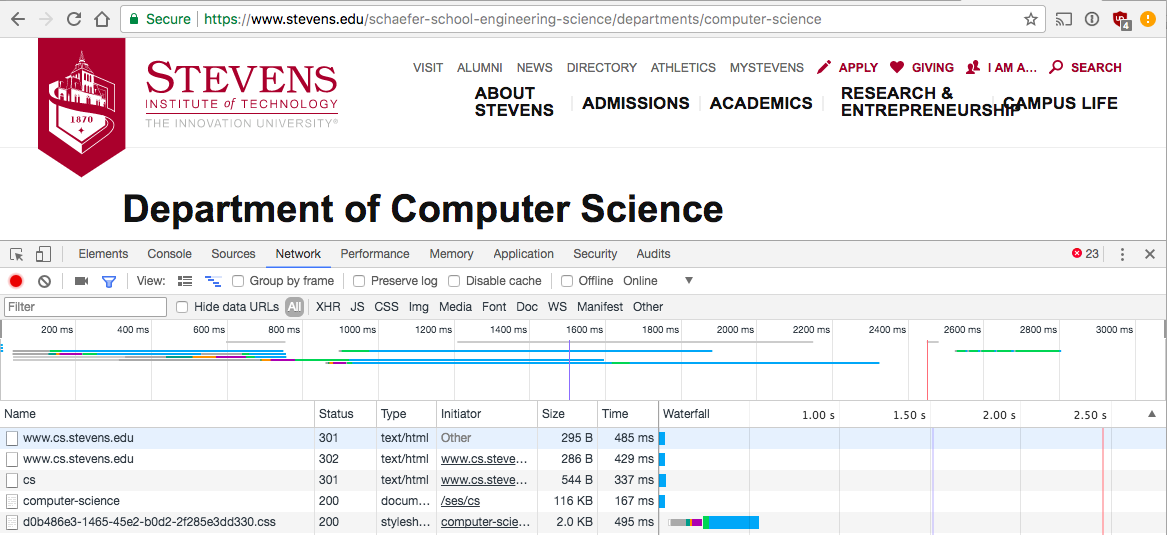
\includegraphics[scale=0.6]{pics/www.cs.stevens.edu.eps}
\end{center}


\subsection{HTTP - more than just text}
HTTP is a {\em Transfer Protocol} -- serving {\em data}, not any specific
text format.

\begin{itemize}
	\item {\tt Accept-Encoding} client header can specify different formats
		such as {\em gzip}, {\em Shared Dictionary Compression over HTTP (SDCH)} etc.
	\item corresponding server headers: {\tt Content-Type} and
		{\tt Content-Encoding}
\end{itemize}
\begin{center}
	
\includegraphics[scale=2.0]{pics/datatransfer.eps}
\end{center}

\subsection{HTTP - more than just static data}
HTTP is a {\em Transfer Protocol} -- what is transferred need not be
static; resources may generate different data to return based on many
variables.

\begin{itemize}
	\item CGI -- resource is {\em executed}, needs to generate
		appropriate response headers
	\item server-side scripting (ASP, PHP, Perl, ...)
	\item client-side scripting (JavaScript/ECMAScript/JScript,...)
	\item applications based on HTTP, using:
		\begin{itemize}
			\item AJAX
			\item RESTful services
			\item JSON, XML, YAML to represent state and
				abstract information
		\end{itemize}
\end{itemize}

\subsection{HTTP in your final project}
\begin{itemize}
	\item protocol versions supported: 1.0
	\item request methods supported: GET, HEAD
	\item request headers supported: If-Modified-Since
	\item response headers included: Date, Server, Last-Modified, Content-Type, Content-Length
\end{itemize}

\subsection{HTTP in your final project}
\begin{itemize}
	\item accept connections, read input from client
	\item timeout idle connections
	\item parse and validate input
	\item generate proper HTTP codes
	\item log connection information
	\item send headers
	\item send response
	\item close connection
\end{itemize}

\subsection{HTTP in your final project}
Client data parsing: \\
\begin{verbatim}
method uri protocol
<optional headers>

\end{verbatim}
\begin{itemize}
	\item {\em method} not in GET, HEAD? \verb+=>+ 400
	\item protocol \verb+!=+ "HTTP/1.0"? \verb+=>+ 505
	\item uri too long? \verb+=>+ 400
\end{itemize}

\subsection{HTTP in your final project}
URI processing:
\begin{itemize}
	\item begins with "/\~{}something"? \verb+=>+ userdir handling
	\item begins with "/cgi-bin/"? \verb+=>+ cgi handling
	\item avoid breaking out of docroot via "../../" etc.
	\item ends in "/"? \verb+=>+ look for 'index.html' or generate index on the fly
\end{itemize}

\subsection{HTTP in your final project}
\verb+https://www.cs.stevens.edu/~jschauma/631/test-sws.sh+

\newpage
\vspace*{\fill}
\begin{center}
	\Hugesize
		Coding Practices\\ [1em]
	\hspace*{5mm}
	\blueline\\
	\hspace*{5mm}\\
		Beyond the Unix Philosophy
\end{center}
\vspace*{\fill}


\subsection{The Unix Philosophy}
\begin{center}
\begin{em}
This is the Unix philosophy:\\
\vspace{.5in}
Write programs that do one thing and do it well. \\

\vspace{.5in}
Write programs to work together. \\

\vspace{.5in}
Write programs to handle text streams,\\
because that is a universal interface.
\end{em}
\end{center}

\subsection{Unix basics}
Write your code and tools such that they work well
within the Unix ecosystem:
\begin{itemize}
	\item write portable code, target different Unix flavors
	\item use \verb+strerror(3)+/\verb+perror(3)+
	\item errors go to \verb+stderr+
	\item use meaningful return codes
	\item follow Unix conventions when using e.g. flags, files, config files, passwords, environment variables, ...
\end{itemize}

\subsection{Unix basics}
Not like this:
\begin{verbatim}
$ hfrob frumbl
Something error ocured!
$ echo $?
0
\end{verbatim}
\vspace{.5in}
But like this:
\begin{verbatim}
$ hfrob frumbl
Unable to open file: '/usr/share/hfrob/frumbl': No such file or directory
$ echo $?
1
\end{verbatim}

\subsection{The Zen of Python}
\smallish
\begin{verbatim}
Explicit is better than implicit.
Simple is better than complex.
Complex is better than complicated.
Flat is better than nested.
Sparse is better than dense.
Readability counts.
Special cases aren't special enough to break the rules.
Although practicality beats purity.
Errors should never pass silently.
Unless explicitly silenced.
In the face of ambiguity, refuse the temptation to guess.
There should be one-- and preferably only one --obvious way to do it.
Although that way may not be obvious at first unless you're Dutch.
Now is better than never.
Although never is often better than *right* now.
If the implementation is hard to explain, it's a bad idea.
If the implementation is easy to explain, it may be a good idea.
Namespaces are one honking great idea -- let's do more of those!
\end{verbatim}
\Normalsize

\subsection{Readability counts}
Visual flow:
\begin{itemize}
	\item use spaces/tabs/indentation {\em consistently}
	\item use a standard width terminal (\verb+~+80 chars)
	\item refactor if code wraps / trails off right side
	\item refactor if logic doesn't fit into about one screen height
	\item never repeat the same code block
\end{itemize}

\subsection{Readability counts}
Not like this:
\begin{verbatim}
        if (smCndt) {
                  foo = fncSmthng();
                        if (strcmp(foo->bar, "MUMBLEFRUMBLE") {
                                        if (otherWat
&& frobbleEnabled) {
printf("Something error ocured!\n")
                    exit(0);
}
                                        }
                  else {
                           frbF();
               }
}
\end{verbatim}

\subsection{Readability counts}
But like this:
\begin{verbatim}
void handleFoo(foo_t *foo) {
        if (strncmp(foo->bar, "MUMBLEFRUMBLE", strlen("MUMBLEFRUMBLE")) > 0) {
                if (otherWat && frobbleEnabled) {
                        fprintf(stderr, "Unexpected value '%s'.", foo->bar);
                }
        }
}

[...]
        if (condition) {
                if ((foo = createFoo()) != NULL) {
                        handleFoo(foo);
                } else {
                        frobFoo(foo);
                }
        }
\end{verbatim}


\subsection{Readability counts}
Code is language:
\begin{itemize}
	\item you are not charged per character
	\item use {\em descriptive} function and variable names
	\item use comments {\em where necessary}; explain {\em why}, not {\em what}
	\item don't use magic numbers
	\item write boring code
\end{itemize}

\subsection{Structure}
\begin{itemize}
	\item "do one thing and do it well" also applies to functions
	\item eliminate side-effects
	\item minimize the use of global variables
	\item keep \verb+open(2)+/\verb+close(2)+, \verb+malloc(3)+/\verb+free(3)+,
		etc. in same (visual/logical) scope
	\item separating code into multiple files helps clarify your interfaces
\end{itemize}

\subsection{Pitfalls}
\begin{itemize}
	\item check the return value of any function that can fail!
	\item avoid file I/O whenever possible
	\item avoid using temporary files whenever possible
	\item don't assume you can write to the current working directory
	\item be explicit in setting permissions; set/use \verb+umask(2)+
	\item use an exit handler to clean up after yourself
	\item retain idempotency whenever possible
\end{itemize}

\subsection{Never trust the user}
\begin{itemize}
	\item your tool must be safe even if hostile input is given
	\item never trust the environment
	\item sanitize and validate all input
	\item you can't exhaustively identify all "bad" cases, so use a whitelist, not a blacklist
\end{itemize}

\subsection{How to figure things out}
\begin{itemize}
	\item know your editor (tags, folds, jumping, ...)
	\item use a debugger
	\item use the source
	\item use \verb+strace(1)+/\verb+dtrace(1)+/\verb+ktrace(1)+ etc.
	\item write separate code to prove yourself right (or wrong)
\end{itemize}

\subsection{Reading}
HTTP etc.:
\begin{itemize}
	\item RFC 2616, 2818, 3875
	\item \verb+http://httpd.apache.org/docs/+
	\item \verb+http://www.w3.org/Protocols/+
	\item REST: \verb+http://is.gd/leSvGa+
\end{itemize}
\vspace{.5in}
Coding practices:
\begin{itemize}
	\item \verb+https://is.gd/xIfOgI+
	\item \verb+https://is.gd/nXh3Pq+
\end{itemize}
\end{document}
